\raggedright
\titledquestion{DFS went wrong!}[6]
The following algorithm which runs DFS on a directed graph, but it contains a fatal error.
\begin{lstlisting}
    Create a stack.
    Choose the initial vertex and mark it as visited.
    Put the initial vertex onto the stack.
    while the stack is not empty:
        Pop a vertex V from the top of the stack.
        for each neighbor of V:
            if that neighbor is not marked as visited:
                Mark that neighbor as visited.
                Push that neighbor onto the stack.
\end{lstlisting}

    
Please give a graph as an counterexample and briefly explain why this algorithm is wrong. 
\\
\textit{Note: In this problem, we say a node is ``visited" whenever it is marked as visited. Pay special attention to how this method differs from the standard DFS in terms of the order in which nodes are marked as visited.}\\


\raggedright
\begin{solution}
    \begin{center}
        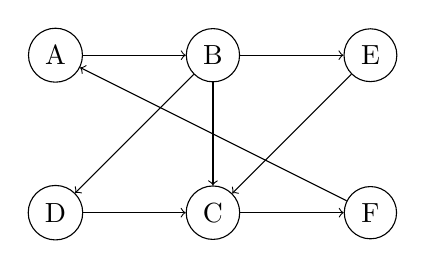
\begin{tikzpicture}[node distance=2cm]
            \node[circle, draw] (A) {A};
            \node[circle, draw, right of=A] (B) {B};
            \node[circle, draw, right of=B] (C) {E};
            \node[circle, draw, below of=A] (D) {D};
            \node[circle, draw, right of=D] (E) {C};
            \node[circle, draw, right of=E] (F) {F};
        
            \draw[->] (A) -- (B);
            \draw[->] (B) -- (C);
            \draw[->] (B) -- (D);
            \draw[->] (B) -- (E);
            \draw[->] (D) -- (E);
            \draw[->] (E) -- (F);
            \draw[->] (F) -- (A);
            \draw[->] (C) -- (E);
        \end{tikzpicture}
        \\
        \vspace{1pt}
    Here we give a counterexample. The graph is shown above. \\
    The initial vertex is A, and we push the neighbors into the stack by lexicographical order in both algorithm.\\

    By the wrong dfs algorithm, the order of visiting the nodes is A, B, E, D, C, F. 
    The correct order should be A, B, E, C, F, D if we perform the right dfs algorithm.\\
    \vspace{1pt}
    The error is made because we mark the node as visited when we find it is a neighbor of the current node, not when we actually visit it. This leads to the wrong order of visiting the nodes, especially when there is an edge between two nodes which are neighbors of another same node.
    \end{center}
\end{solution}